\section{Experiments}
We setup two environments in the grid world and windy grid world.

\subsection{Four room grid world}
Four room grid world is a grid world with four rooms connected to each other as shown in Figure~\ref{fig:four-room-grid-world}.

\subsection{Four room windy world}

Four room windy world is a grid world with four rooms connected to each other as shown in Figure~\ref{fig:four-room-grid-world}.
Some of the grid cells in have wind shown by arrow and the agent gets pushed around by
the wind with 0.25 probability irrespective of the action taken.

\subsection{Metrics}
We describe the metrics used to quantify and compare agent performance
in these environments.

\begin{enumerate}
    \item \textbf{Reward}\\\noindent
        As in typical in reinforcement learning, the reward earned by
        the agent is treated as a metric of success. Since the
        environments used are finite MDPs, Q-Learning is known to learn
        the optimal policy given enough exploration time. 

    \item \textbf{\Loo}\\
        First defined in \cite{MiPaViICLR2017}, \Loo is the ratio of the
        amount of time taken to hit the goal for the first time to the
        average amount of time taken to hit goals subsequently. It is
        the ratio of the exploration time over the exploitation time. 

    \item \textbf{Distance-Inefficiency}\\
        Introduced in \cite{dhiman2018critical}, the
        distance-inefficiency is the ratio of the distances travelled by
        the agent during an episode to the sum of the shortest path to
        the goal at every point of initialization. 
\end{enumerate}


%
\begin{figure}%
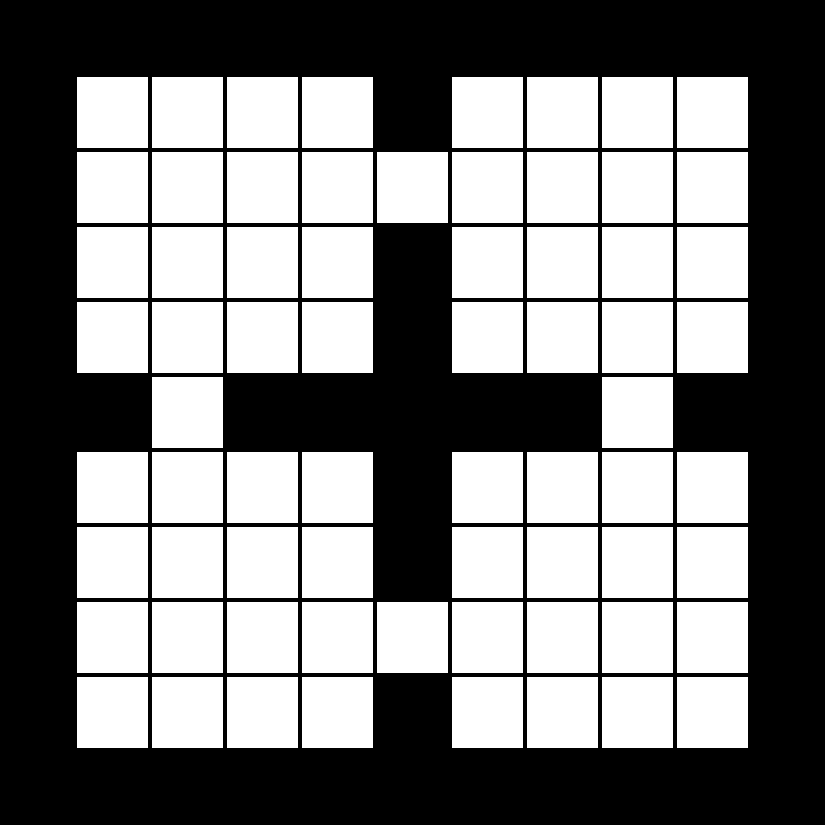
\includegraphics[width=0.48\columnwidth]{media/4-room-grid-world.pdf}
\hfill
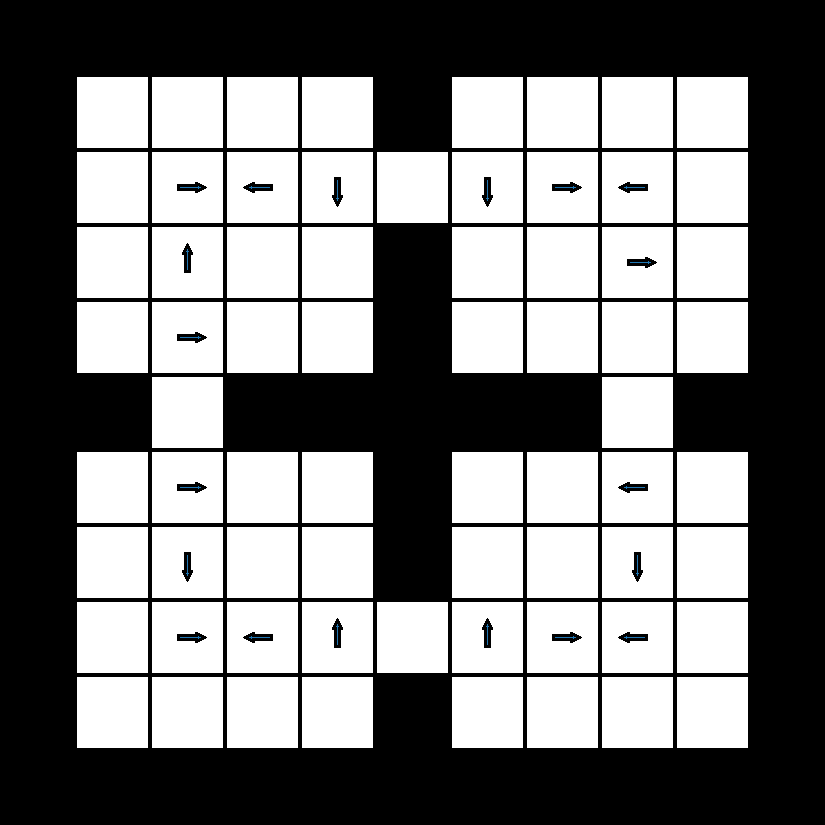
\includegraphics[width=0.48\columnwidth]{media/4-room-windy-world.pdf}%
\caption{Left: Four room grid world. Right: Four room windy grid world with wind direction shown by arrows. The windy pushes the agent in the direction of wind with 0.25 probability irrespective of the action taken.}
\label{fig:four-room-grid-world}%
\end{figure}%

